\chapter{Conceptdimensionering}
%In dit hoofdstuk: kritische onderdelen, maak- en koopdelen, toleranties, verbeterde SW-model.
\label{Concept_dimensionering}
\textit{In dit hoofdstuk wordt er verder gekeken naar de specifieke concept-dimensionering. Hierbij worden de kritische onderdelen vastgesteld en vervolgens berekent op sterkte en stijfheid (\cref{se:kritische_onderdelen}). Uit deze berekeningen volgen de dimensies. \\
Als de dimensies zijn afgerond wordt er een maak- en kooplijst gemaakt. Bij het opstellen van deze lijsten wordt er rekening gehouden met de geometrie, dimensies en materiaalkeuze op basis van de berekeningen.}


\section{Kritische onderdelen.}
\label{se:kritische_onderdelen}
In dit deel van het hoofdstuk wordt gekeken naar welke onderdelen mogelijke kritische onderdelen zijn en de dimensionering ervan. Eerst worden de kritische onderdelen vastgesteld en worden er aannames gemaakt over hoe deze onderdelen worden belast \cref{se:onderdelen_met_toelichting}. In \cref{se:werking_kritische_onderdelen} worden de kritische onderdelen verder toegelicht. Er wordt kort verteld hoe ze in elkaar zitten en werken. In \cref{se:berekening_en_dimensionering} wordt er gekeken naar de dimensionering en worden de berekeningen aan de verschillende kritische onderdelen uitgewerkt.
\vspace{1mm}

\subsection{De onderdelen met toelichting.}
\label{se:onderdelen_met_toelichting}
De onderdelen die de grootste kans op falen hebben zijn:

\begin{description}
    \item \textbf{De wielassen.} De keuze van de wielassen als kritisch onderdeel is gemaakt vanwege het grote gewicht dat op de assen komt te staan. Een as moet vanwege de werking van het pakket hondje tijdens het nemen van het talud de helft van het totale gewicht kunnen hebben. \\

    \item \textbf{De schaarliften.} Dit onderdeel is essentieel voor de werking van het mechanisme. De krachten op de members van de schaarlift zijn mogelijk erg groot, daarom is het nodig om te kijken welke krachten spelen in deze members om ze goed te kunnen dimensioneren.\\

    \item \textbf{De motoren.}
    
    \item \textbf{Het stuursysteem.} Voor het verloop van het parcours is het van belang er bochten gemaakt kunnen worden, dit wordt gedaan met het Ackermann stuursysteem. Door vele bewegende onderdelen is het van belang dat dit niet bezwijkt onder druk, ook moet er berekend worden of de scherpe hoek kan worden gemaakt (met eventueel paar keer steken).\\
    
    \item \textbf{L-profiel aan de bovenkant van de kar.}

    \item \textbf{U-profiel aan de onderkant van de kar.} Aan de onderkant van de kar moeten de schaarliften worden bevestigd samen met de motoren en de wielen. Dit onderdeel moet dus goed op stijfheid worden gedimensioneerd omdat het essentieel is dat dit onderdeel niet vervormd met alle gevolgen van dien.\\ 
\end{description}

\vspace{\baselineskip}
\subsection{Werking en functie kritische onderdelen.}
\label{se:werking_kritische_onderdelen}

\textbf{De wielassen.}\\
Aan de onderkant van het pakket hondje hebben wij wielen gemaakt, deze wielen worden op hun plek gehouden door middel van assen. Deze assen worden aangedreven en moet er voor zorgen dat het pakkethondje zich voortbeweegt.\\
\vspace{\baselineskip}

\textbf{De schaarliften.}\\
Een essentieel onderdeel voor de werking van ons talud-neem-mechanisme zijn de schaarliften. Door een schaarlift op te klappen en die over het talud te rijden is het pakket hondje in staat om als het ware over het talud te stappen.\\
\vspace{\baselineskip}

\textbf{De motoren}

\textbf{Ackermann-stuursysteem.}\\
Bij het ackermann stuursysteem wordt er uitgegaan van het Ackermann principe: de wielen op de as maken altijd een hoek van 90 graden ten opzichte van een bepaald punt wat achter de as ligt. De wielen moeten met behulp van fusees zijn bevestigd met de wielas, omdat de starre as niet kan meedraaien en dit ook niet de bedoeling is. De fusees zijn verbonden met een andere as, niet de wielas, welke voor de uiteindelijke draairichting zorgt, zie \cref{fig: ackermann_FBD}. Deze as wordt aangedreven d.m.v. een servomotor en zo kan de bochtstraal/bocht richting worden bepaald. Deze servo is niet weergegeven in \cref{fig: ackermann_FBD} maar zal wel in ons concept komen. De bochtstraal hangt ook af van de achterste wielas. Deze wielen draaien niet mee en dus wordt er voor de bochtstraal uitgegaan van de hartlijn van de achterwielen. De wielen dienen minimaal zodanig te draaien dat ze loodrecht staan op het punt waar je omheen wil draaien, in de afbeelding de ‘centre of turning’.\\

\begin{figure}[H]
    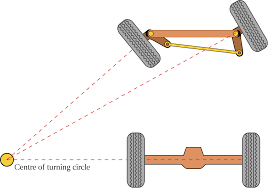
\includegraphics[width = 100mm]{04_conceptdimensionering/ackermann.png}
    \caption{Ackermann Stuursysteem, }
    \label{fig: ackermann_FBD}
\end{figure}
\vspace{1mm}

\textbf{L-profiel aan de bovenkant van de kar.}

\vspace{1mm}
\textbf{U-profiel aan de onderkant van de kar.}\\
De wielassen en de schaarliften moeten aan elkaar worden bevestigd, dit doet het u-profiel aan de onderkant van de kar. Hier worden ook de motoren bevestigd die de wielassen aandrijven.\\

\vspace{1mm}
\subsection{Berekeningen en dimensionering}
\label{se:berekening_en_dimensionering}
\vspace{\baselineskip}

\textbf{De wielassen}.\\
Er is gerekend aan de assen en de conclusie is dat een 6/8 mm as van staal voldoet. De berekening is gemaakt in een python script, zie \cref{Cha:Bijlage_F}.\\
\vspace{\baselineskip}
De berekening is als volgt opgezet:\\
Om aan de situatie te kunnen rekenen, moest eerst de situatie versimpeld worden en tot een reëel FBD worden gebracht, zie \cref{fig: as_FBD}. Hier is aangenomen dat je de as kan beschouwen als een aan twee kanten ingeklemde balk. Ook is F niet P, door een verdeling van gewicht. Deze verdeling is bekend.

\begin{figure}[H]
    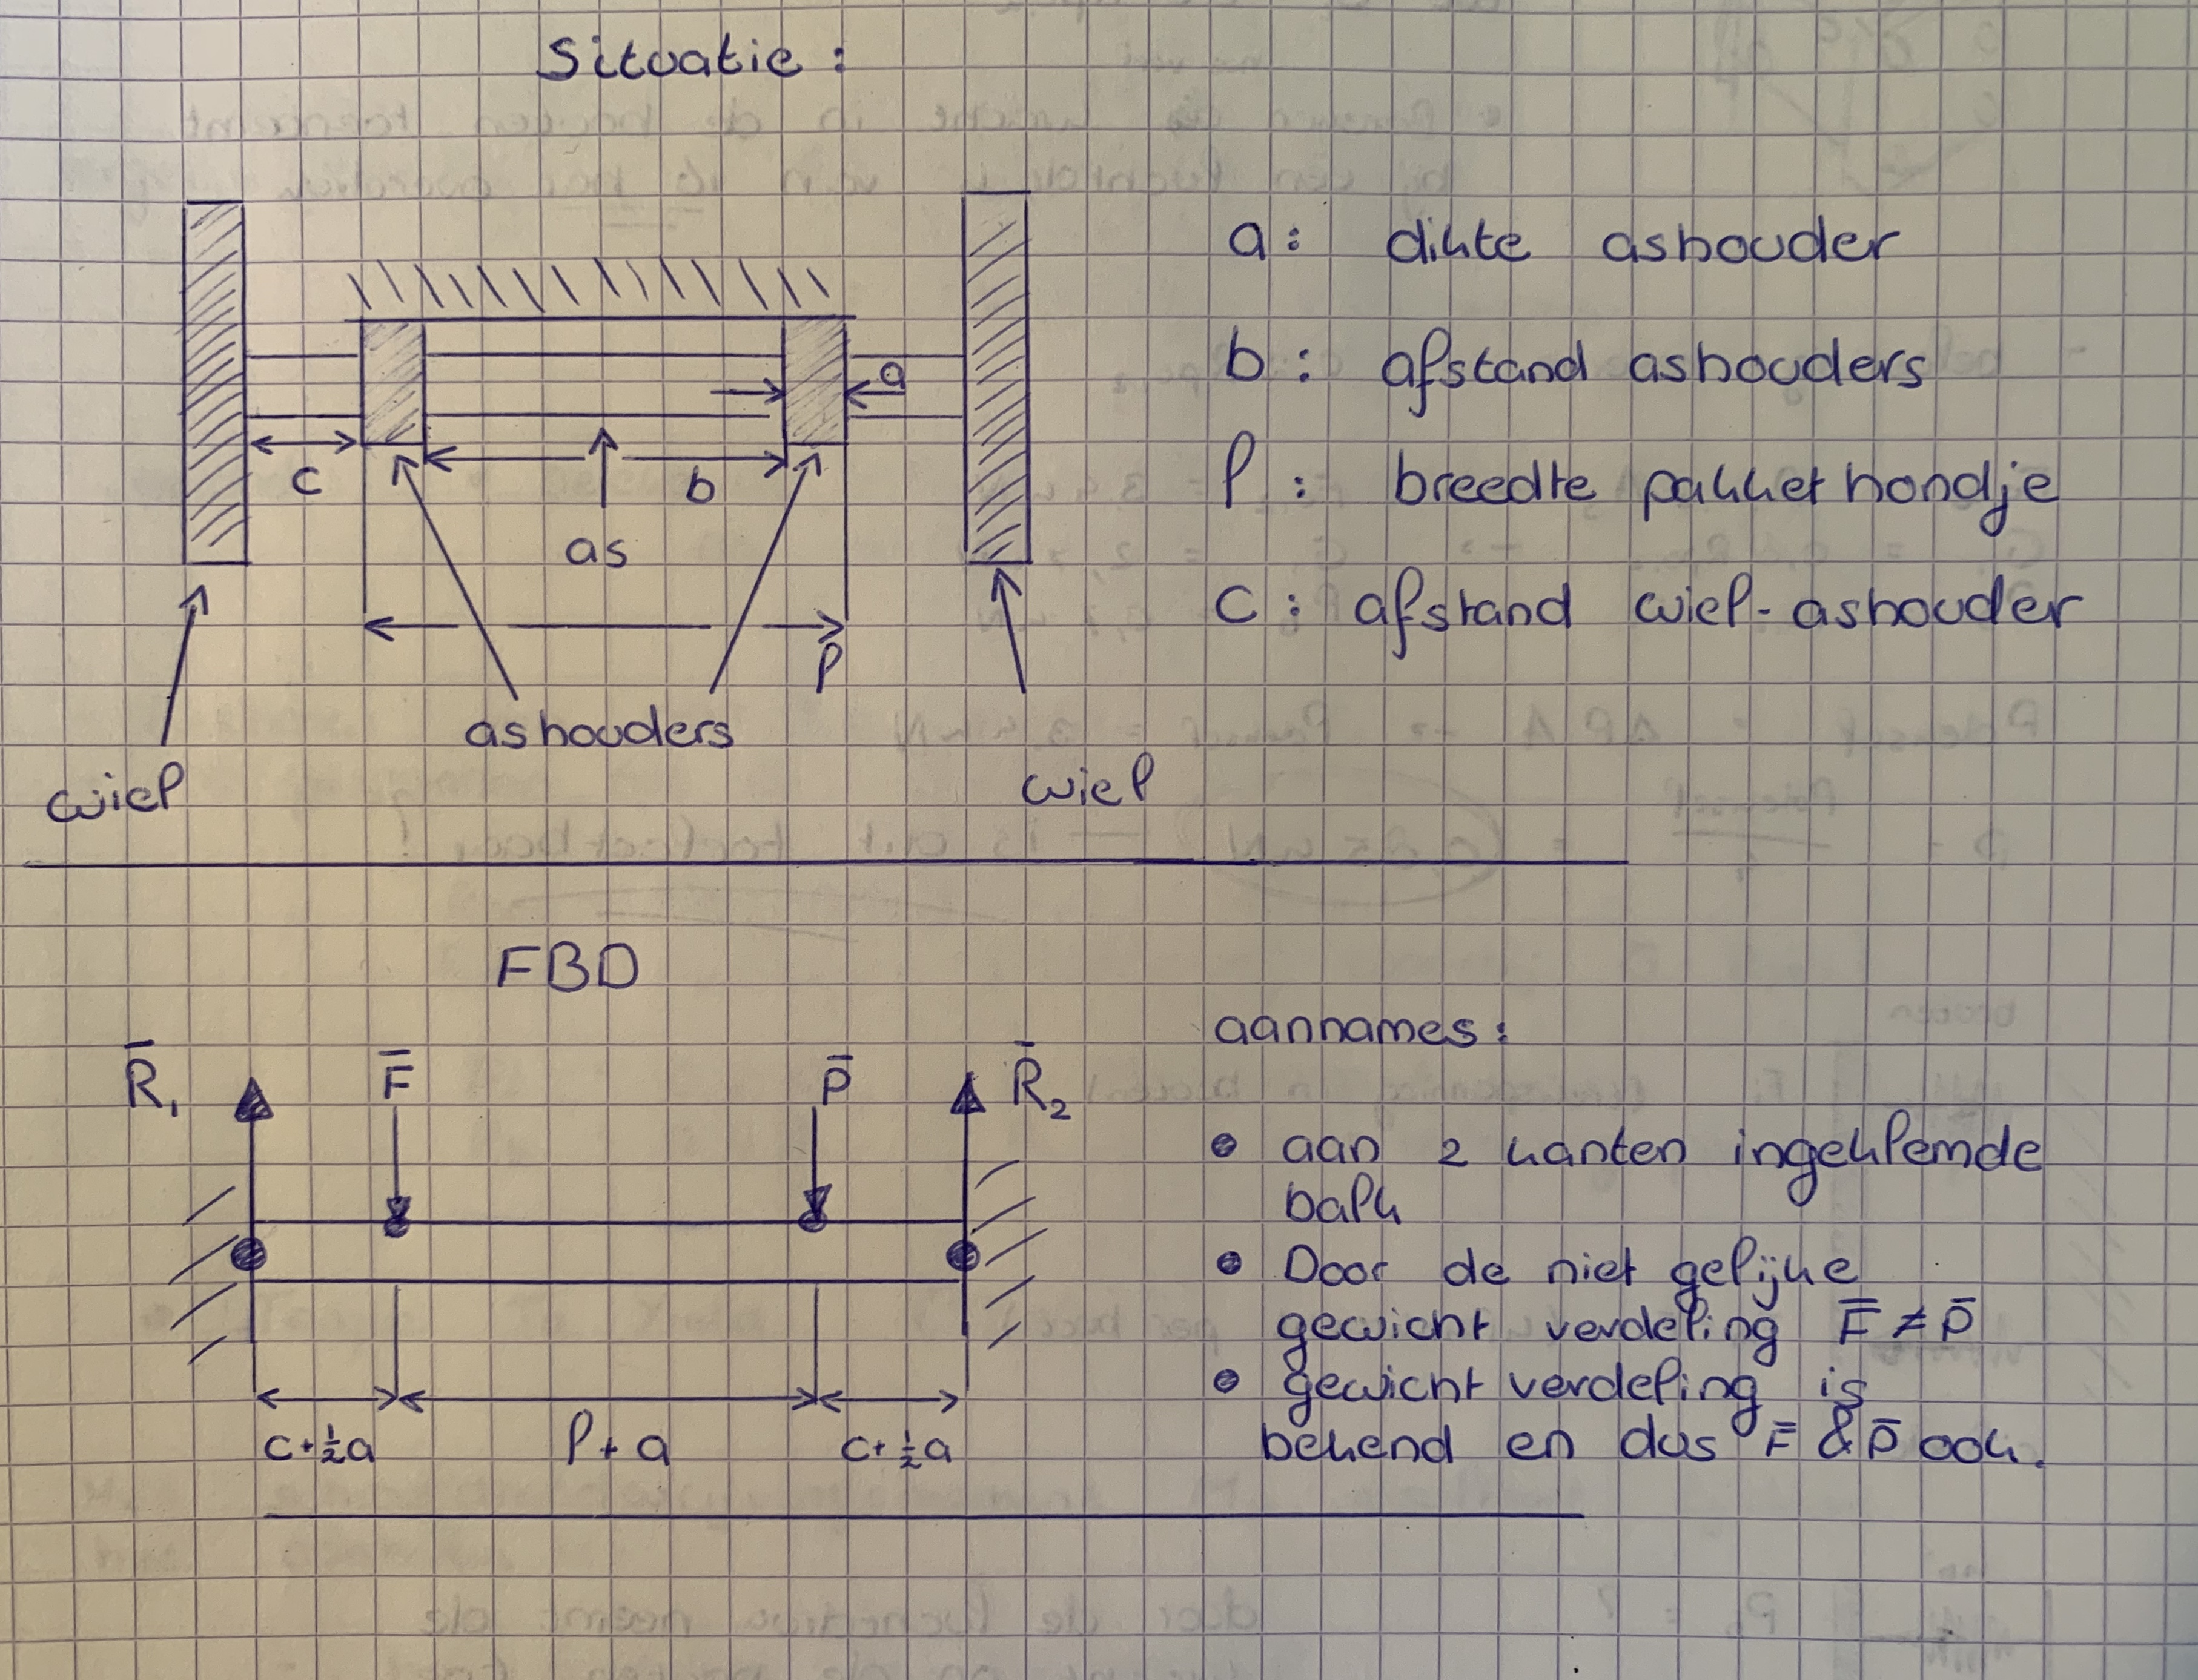
\includegraphics[width = 100mm]{04_conceptdimensionering/As_FBD.jpg}
    \caption{Bepaling van het FBD van de as.}
    \label{fig: as_FBD}
\end{figure}

Door middel van de snede methode kan je vervolgens de krachten en momenten lijn opstellen, deze berekening is te zien in \cref{Cha:Bijlage_F}. In \cref{fig: as_constanten} zijn de constanten te zien die zijn gebruikt voor het bepalen van de momenten en krachten lijn. Deze constanten hebben geleid tot de momenten en krachten lijn die te zien zijn in \cref{fig: Momentenlijn_as} en \cref{fig: Krachtenlijn_as}. \\

\begin{figure}[H]
    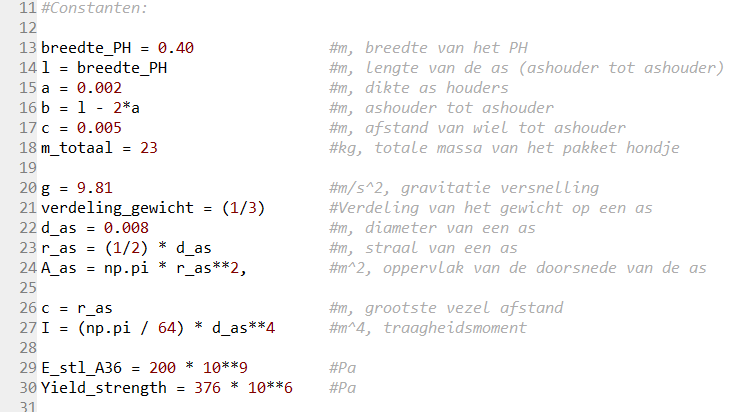
\includegraphics[width = 100mm]{04_conceptdimensionering/Constanten_as_goed.PNG}
    \caption{Constanten van de as.}
    \label{fig: as_constanten}
\end{figure}

\begin{figure}[H]
    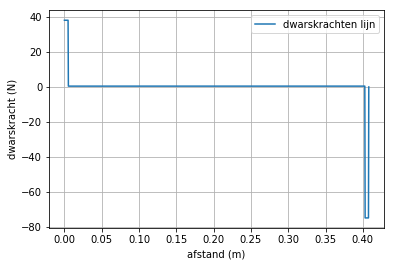
\includegraphics[width = 100mm]{04_conceptdimensionering/Krachtenlijn_as.png}
    \caption{Krachten lijn in de as.}
    \label{fig: Krachtenlijn_as}
\end{figure}

\begin{figure}[H]
    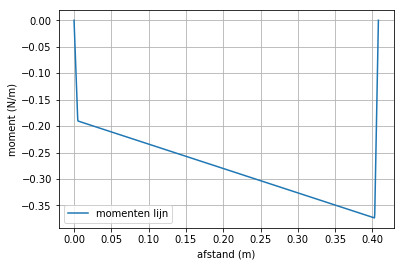
\includegraphics[width = 100mm]{04_conceptdimensionering/Momentenlijn_as.png}
    \caption{Momenten lijn in de as.}
    \label{fig: Momentenlijn_as}
\end{figure}


\textbf{De schaarliften.}\\
Ook aan de schaarliften zijn gerekend en de conclusie is dat de schaarliften een koker-profiel krijgen, met dit profiel en een gepaste lengte kan een member van de schaarlift de krachten hebben.\\
Voor de schaarliften is naar een aantal dingen gekeken:\\
\vspace{\baselineskip}
\begin{enumerate}
    \item \textbf{De vorm van belasting.} Er is een FBD van de schaarlift en van een members opgesteld om te kijken naar de vorm van de belasting op de onderdelen, zie \cref{fig: FBD_member}. Uit deze FBD kan worden geconcludeerd dat de members van de schaarlift op zuivere druk worden belast. Hierdoor moet rekening worden gehouden met knik en met de druksterkte van het materiaal.\\
    \item \textbf{De mate van belasting.} Om te bepalen wat de grootte van de belasting is moeten de krachten worden ontleden. Gebleken is na onderzoek door middel van een python script (\cref{se: bijlage_F schaarliften}) dat de members de belasting kunnen hebben. Uit het script worden bepaalde conclusies getrokken die te vinden zijn in \cref{fig: Kernel_schaarlift_1} en \cref{fig: Kernel_schaarlift_2}.\\
    \item \textbf{Het profiel van de members.} Uit het onderzoek is gebleken dat de members op een zuivere druk worden belast. Dit betekend dat er niet voor een specifiek profiel hoeft worden gekozen mits het oppervlak van een doorsnede groot genoeg is. Toch hebben wij voor een koker-profiel gekozen omdat naast de verwachtte krachten langs de members het ook waarschijnlijk is dat er krachten zullen opspelen in andere richtingen. Daarom is voor de zekerheid gekozen voor een koker profiel met de dimensionering% die te vinden is in \cref{fig:schaarliften_constanten} in \cref{se: bijlage_F schaarliften}
    . Ook zijn hier berekeningen mee gedaan die te vinden zijn in \cref{fig: Kernel_schaarlift_2}.\\
    \item \textbf{De dimensionering van de members.} De dimensionering van de members zijn uit het python script gehaald, die zijn te vinden in %\cref{fig:schaarliften_constanten} en in 
    \cref{fig: Kernel_schaarlift_1}.
\end{enumerate}
\vspace{\baselineskip}

\begin{figure}[H]
    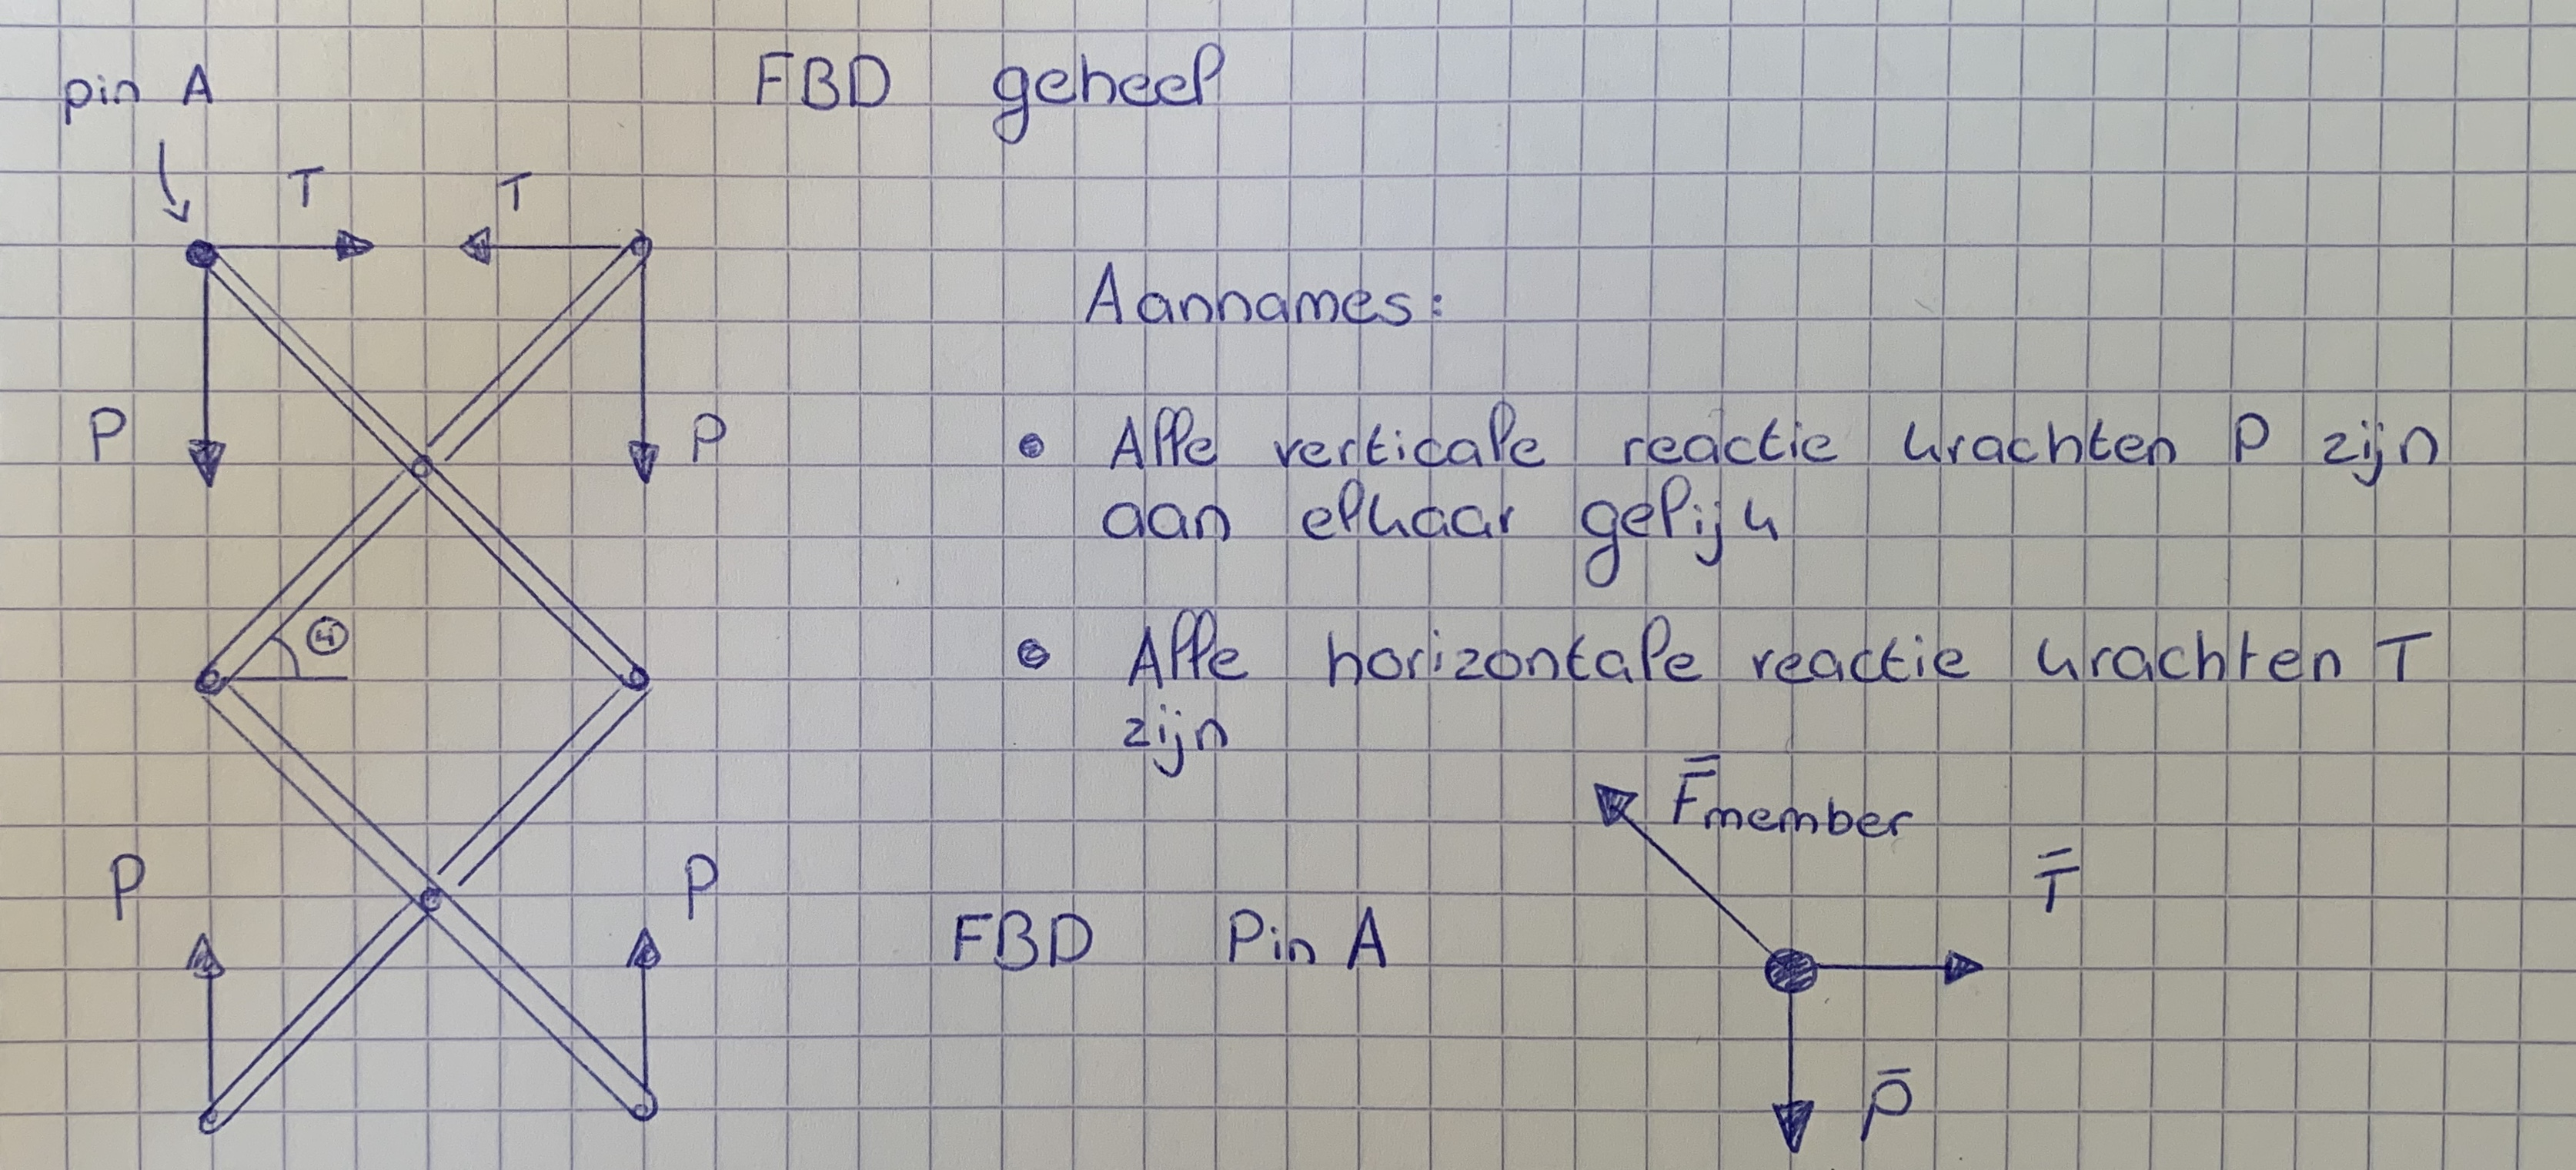
\includegraphics[width = 100mm]{04_conceptdimensionering/member_FBD.jpg}
    \caption{FBD van de schaarlift en pin in een member.}
    \label{fig: FBD_member}
\end{figure}
\vspace{\baselineskip}

\begin{figure}[H]
    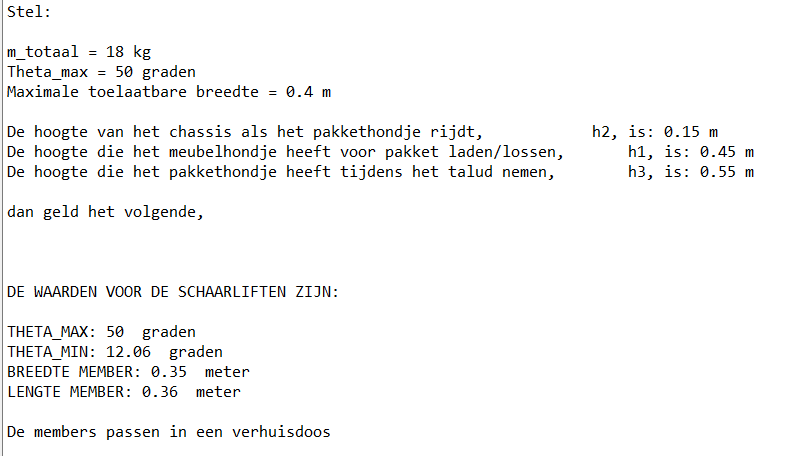
\includegraphics[width = 100mm]{04_conceptdimensionering/Schaarlift_kernel_1.PNG}
    \caption{Kernel van het python script.}
    \label{fig: Kernel_schaarlift_1}
\end{figure}

\begin{figure}[H]
    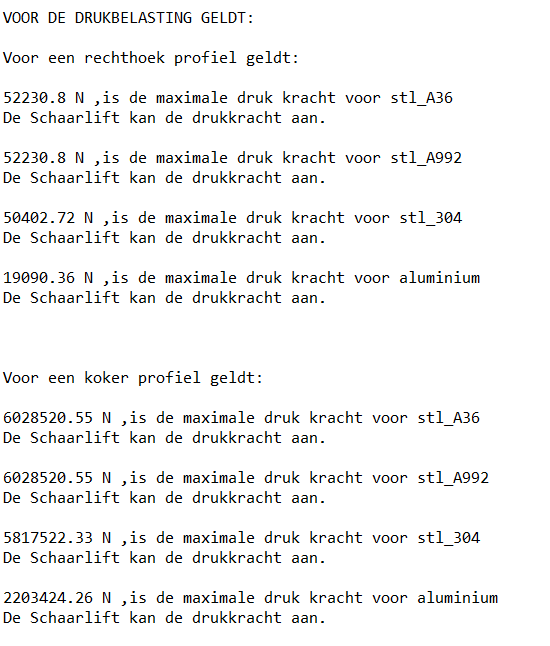
\includegraphics[width = 80mm]{04_conceptdimensionering/Schaar.PNG}
    \caption{Kernel van het python script.}
    \label{fig: Kernel_schaarlift_2}
\end{figure}
\vspace{\baselineskip}

\textbf{De motoren.}\\

\textbf{Het stuursysteem.}\\

\textbf{L-profiel aan de bovenkant van de kar.}\\

\textbf{U-profiel aan de onderkant van de kar.}\\
Er is voor een U-profiel gekozen vanwege de vorm van de belasting. Deze is versimpeld weergegeven in \cref{fig: schets_FBD_uprofiel} te zien. Wanneer de zijkanten als ingeklemd worden beschouwd kan de conclusie worden getrokken dat het onderdeel zowel op buiging als op trek wordt belast. Een geschikt profiel voor dit soort belasting is het U-profiel.\\
Hiermee is een python script geschreven, zie \cref{se: onderkant_u-profiel} in \cref{Cha:Bijlage_F}. Uit dit script is de dimensionering gehaald%, zie \cref{fig:u-profiel_constanten}
. Het u-profiel is vervolgens berekend op sterkte en stijfheid er is een krachten- en momentenlijn opgesteld (\cref{fig: momentenlijn_onderkant} \& \cref{fig: krachtenlijn_onderkant}). Uit de momenten en krachtenlijn is gebleken dat het u-profiel de krachten kan hebben, zie \cref{fig: kernel_onderkant}.

\begin{figure}[H]
    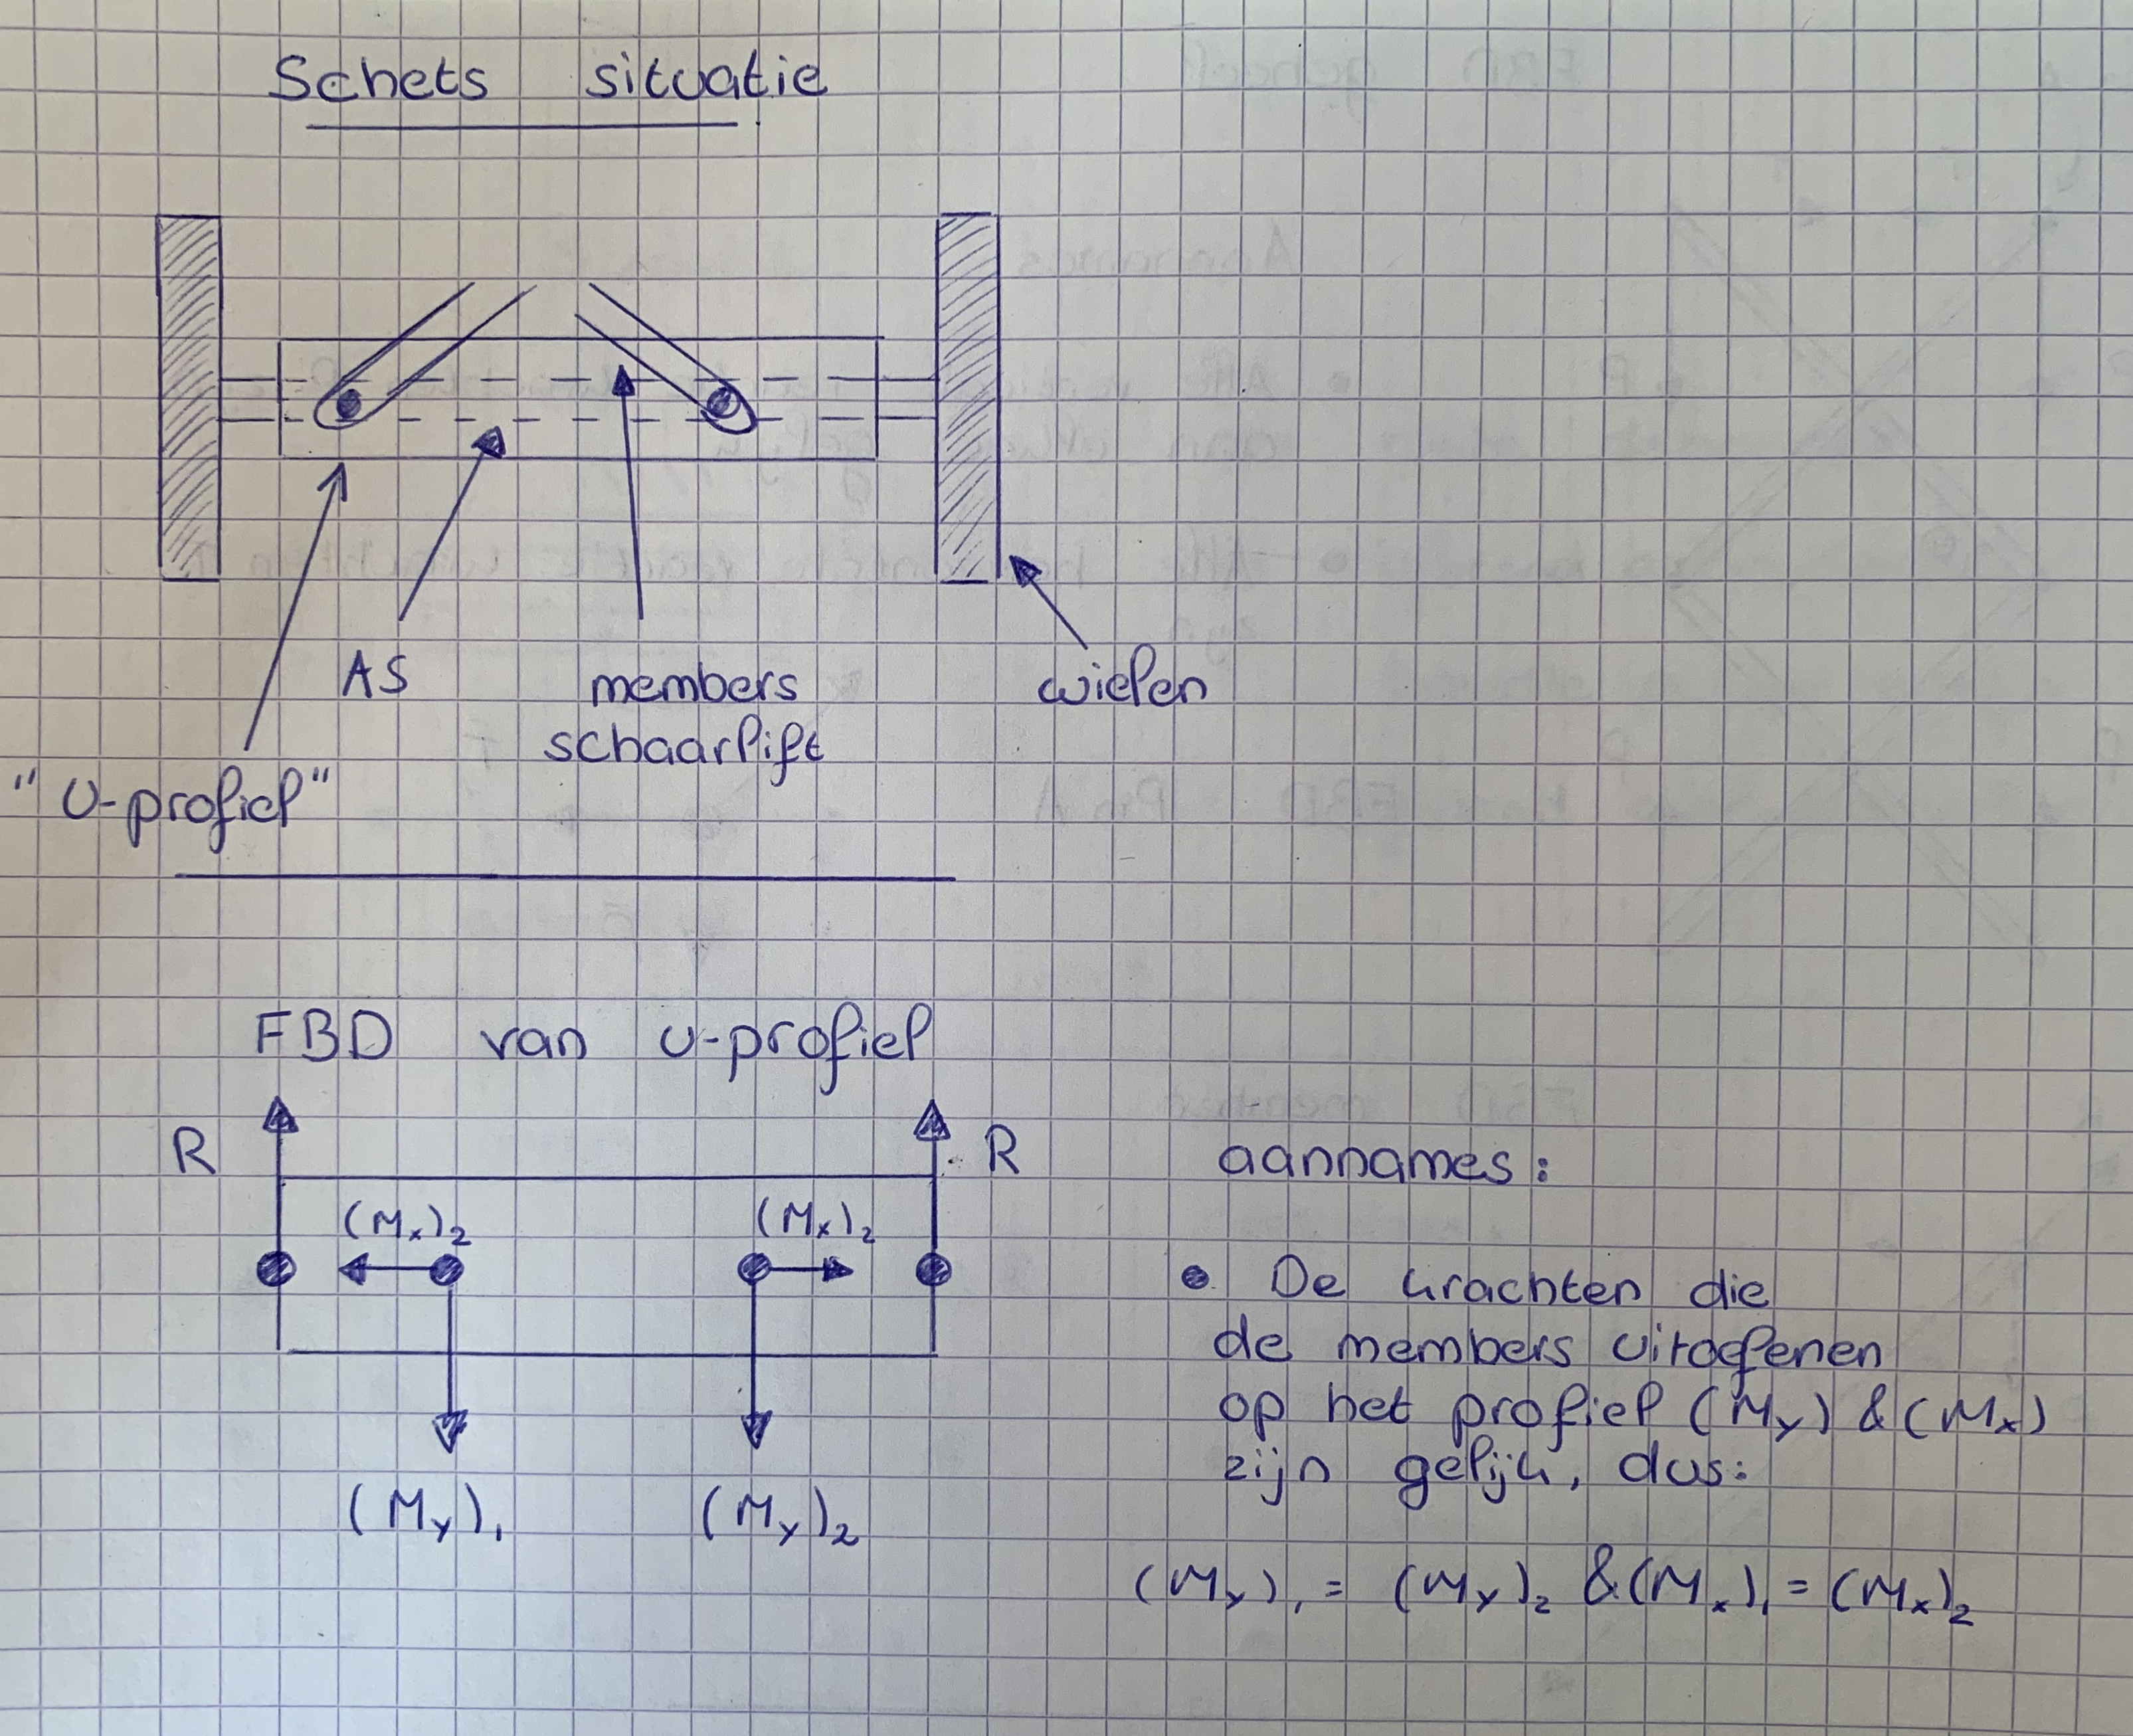
\includegraphics[width = 80mm]{04_conceptdimensionering/U-profiel_tekening.jpg}
    \caption{schets situatie en FBD van u-profiel onderaan de kar.}
    \label{fig: schets_FBD_uprofiel}
\end{figure}
\vspace{\baselineskip}

\begin{figure}[H]
    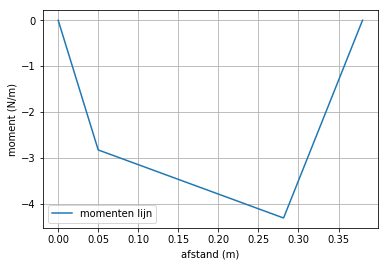
\includegraphics[width = 80mm]{06_bijlage_F/onderkant_u_profiel/momentenlijn_onderkant.png}
    \caption{Momentenlijn van het u-profiel aan de onderkant van de kar.}
    \label{fig: momentenlijn_onderkant}
\end{figure}
\vspace{\baselineskip}

\begin{figure}[H]
    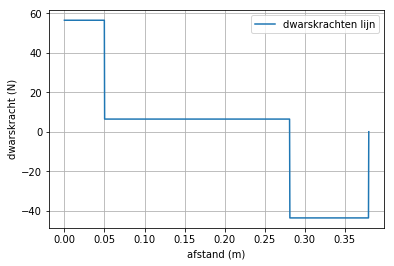
\includegraphics[width = 80mm]{06_bijlage_F/onderkant_u_profiel/krachtenlijn_onderkant.png}
    \caption{Krachtenlijn van het u-profiel aan de onderkant van de kar.}
    \label{fig: krachtenlijn_onderkant}
\end{figure}
\vspace{\baselineskip}

\begin{figure}[H]
    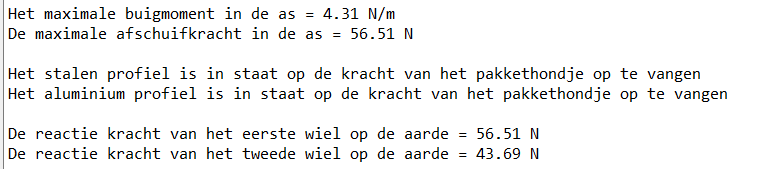
\includegraphics[width = 120mm]{06_bijlage_F/onderkant_u_profiel/kernel_onderkant.PNG}
    \caption{Kernel van het python script.}
    \label{fig: kernel_onderkant}
\end{figure}
\vspace{\baselineskip}










\section{Maak- en kooplijst}
\label{maaklijst_kooplijst}

Nadat de berekeningen en dimensionering zijn afgerond kunnen de maak- en kooplijsten worden opgesteld. In \cref{fig:maaklijst} staat de maaklijst van de driepoter en in \cref{fig:kooplijst} staat de kooplijst van de driepoter.

\begin{figure}[H]
    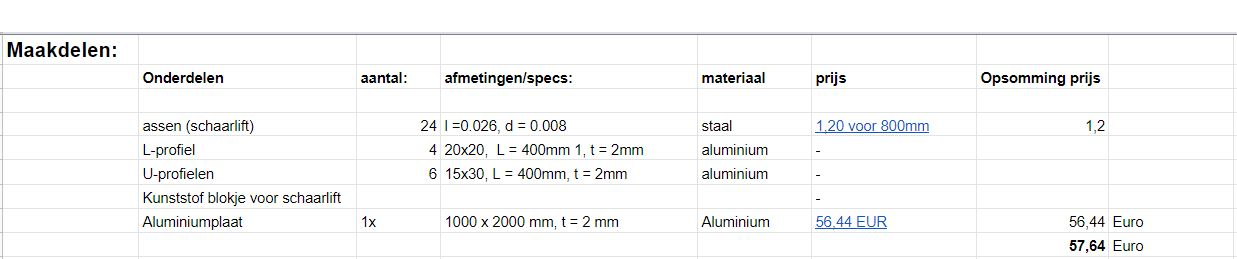
\includegraphics[width = 120mm]{04_conceptdimensionering/Tabel_Maaklijst.JPG}
    \caption{Maaklijst van de Driepoter}
    \label{fig:maaklijst}
\end{figure}

De maaklijst bevat de onderdelen die zelf gefabriceerd kunnen worden, hieronder verstaat men de L-profielen en de U-profielen. Deze profielen worden uit aluminiumplaat gesneden en vervolgens gebogen. 

\vspace{\baselineskip}
\begin{figure}[H]
    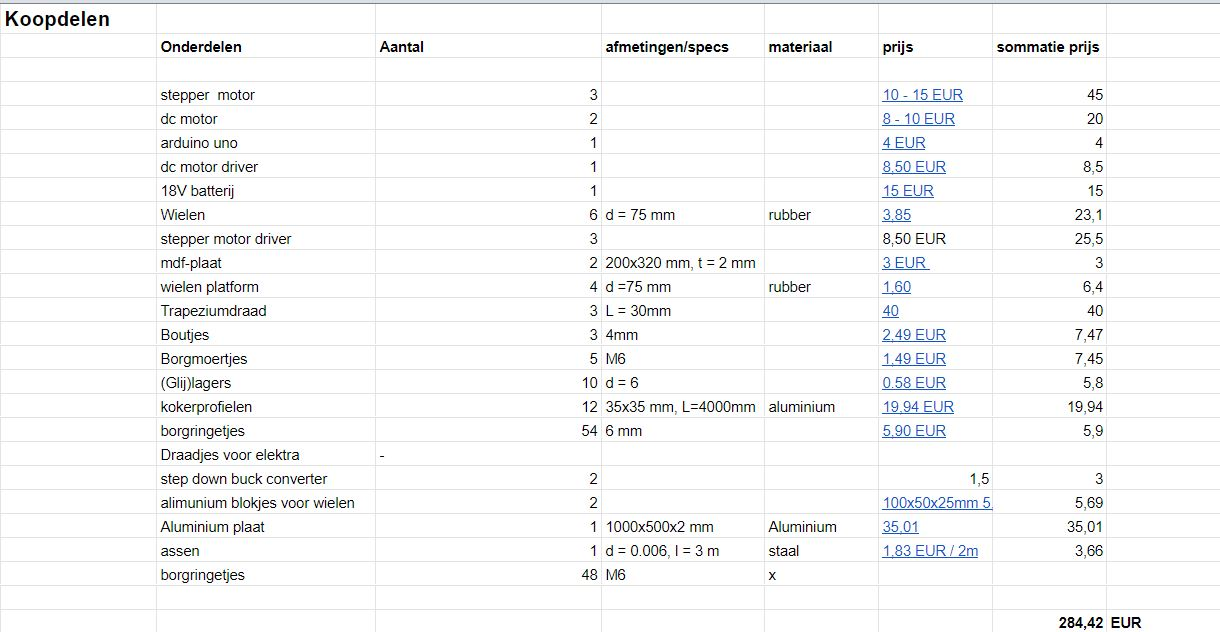
\includegraphics[width = 120mm]{04_conceptdimensionering/Tabel_Kooplijst.JPG}
    \caption{Kooplijst van de Driepoter}
    \label{fig:kooplijst}
\end{figure}

\section{Bestellijst.}
Uit de kooplijst is een selectie gemaakt van onderdelen, die samen maximaal 80 euro kostten. 